%!TEX program = pdflatex
\documentclass[conference,10pt,a4paper]{IEEEtran}

\usepackage[utf8]{inputenc}
\usepackage[T1]{fontenc}
\usepackage[american]{babel}

\usepackage[acronym, nomain, nowarn]{glossaries}
\loadglsentries{acronyms}
\usepackage[hyphens]{url}

\usepackage{mathtools}
\usepackage{fixmath}
\usepackage{algorithm2e}
\usepackage{subcaption}
\usepackage{siunitx}
\usepackage{eurosym}

\DeclareSIUnit\year{yrs}
\DeclareSIUnit{\EUR}{\text{\euro}}
\sisetup{load-configurations = abbreviations,
         binary-units, 
         per-mode=fraction}
\usepackage{csquotes}
\usepackage{booktabs}
\usepackage{tabu}

\makeglossaries

\usepackage[url=false,
            doi=true,
            backend=biber,
            style=ieee,
            isbn=false,
            sorting=none]{biblatex}
\addbibresource{literature.bib}
\usepackage[inline]{enumitem}

\usepackage[np]{numprint}
\npstyleenglish


\usepackage{balance}

\usepackage{xspace}
\newcommand{\steam}{\textsc{Steam}\xspace}
\newcommand{\hltb}{\textsc{How Long To Beat}\xspace}
\newcommand{\metacritic}{\textsc{Metacritic}\xspace}
\newcommand{\gfnow}{\textsc{GeForce NOW}\xspace}
\newcommand{\gfnowpc}{\textsc{GeForce NOW} for \gls{PC}\xspace}
\newcommand{\psnow}{\textsc{PlayStation Now}\xspace}
\newcommand{\psnowpc}{\textsc{PlayStation Now} on \gls{PC}\xspace}
\newcommand{\liquid}{\textsc{LiquidSky}\xspace}


\begin{document}

\title{Subjective And Objective Assessment Of Video Game Context Factors}

\author{\IEEEauthorblockN{Florian Metzger}
\IEEEauthorblockA{
Chair of Communication Networks\\
University of Würzburg, Germany\\
florian.metzger@uni-wuerzburg.de}
\and
\IEEEauthorblockN{Svenja Schröder, Albert Rafetseder}
\IEEEauthorblockA{
Cooperative Systems Research Group\\
Faculty of Computer Science\\
University of Vienna, Austria\\
\{svenja.schroeder|albert.rafetseder\}@univie.ac.at}
}
\maketitle

%!TEX root = paper.tex
%%%%%%%%%%%%%%%%%%%%%%%%%%%%%%%%%%%%%%%%%%%%%%%%%%%%%%%%%%%%%%%%%%%%%%%%%%%%%%%

\newglossaryentry{cg}{name={cloud gaming},description={Gaming in the cloud}}
\newglossaryentry{cr}{name={cloud rendering},description={In contrast to \gls{Gaas}, the game is provided by the customer and is only rendered in the cloud}}

%\newacronym[description={\glslink{2g}{Second Generation}}]{2G}{2G}{Second Generation}
\newacronym{2G}{2G}{Second Generation}
\newacronym{3G}{3G}{Third Generation}
\newacronym{3GPP}{3GPP}{Third Generation Partnership Project}
\newacronym{AAA}{AAA}{Authentication, Authorization and Accounting}
\newacronym{AAC}{AAC}{Advanced Audio Coding}
\newacronym{ABI}{ABI}{Application Binary Interface}
\newacronym{AMBR}{AMBR}{Aggregate Maximum Bit-Rate}
\newacronym{ANOVA}{ANOVA}{Analysis of Variance}
\newacronym{API}{API}{Application Programming Interface}
\newacronym{APM}{APM}{Actions per Minute}
\newacronym{APN}{APN}{Access Point Name}
\newacronym{AQM}{AQM}{Active Queue Management}
\newacronym{ARQ}{ARQ}{Automatic Repeat Request}
\newacronym{ASN.1}{ASN.1}{Abstract Syntax Notation One}
\newacronym{ATM}{ATM}{Asynchronous Transfer Mode}
\newacronym{AU}{AU}{Access Unit}
\newacronym{AuC}{AuC}{Authentication Centre}
\newacronym{AVC}{AVC}{Advanced Video Coding}
\newacronym{BDP}{BDP}{Bandwidth-Delay Product}
\newacronym{BGP}{BGP}{Border Gateway Protocol}
\newacronym{BMC}{BMC}{Broadcast/Multicast Control}
\newacronym{BSC}{BSC}{Base Station Controller}
\newacronym{BSD}{BSD}{Berkeley Software Distribution}
\newacronym{BSS}{BSS}{Base Station Subsystem}
\newacronym{BTS}{BTS}{Base Transceiver Station}
\newacronym{CAMEL}{CAMEL}{Customised Applications for Mobile Networks Enhanced Logic}
\newacronym{CAPEX}{CAPEX}{CAPital EXpenditure}
\newacronym{CCG}{CCG}{Collectible Card Game}
\newacronym{CDF}{CDF}{Cumulative Distribution Function}
\newacronym{CDN}{CDN}{Content Distribution Network}
\newacronym{CDMA}{CDMA}{Code Division Multiple Access}
\newacronym{CELLDCH}{CELL\_DCH}{Dedicated Channel}
\newacronym{CELLFACH}{CELL\_FACH}{Forward Access Channel}
\newacronym{CELLPCH}{CELL\_PCH}{Cell Paging Channel}
\newacronym{CGN}{CGN}{Carrier-grade \acrshort{NAT}}
\newacronym{CI}{CI}{Continuity Index}
\newacronym{CN}{CN}{Core Network}
\newacronym{CPU}{CPU}{Central Processing Unit}
\newacronym{CS}{CS}{Circuit Switching}
\newacronym{CSG}{CSG}{Closed Subscriber Group}
\newacronym{CSS}{CSS}{Cascading Style Sheets}
\newacronym{DANE}{DANE}{DNS-Based Authentication of Named Entities}
\newacronym{DASH}{DASH}{Dynamic Adaptive Streaming over \acrshort{HTTP}}
\newacronym{DCCP}{DCCP}{Datagram Congestion Control Protocol}
\newacronym{DCE}{DCE}{Direct Code Execution}
\newacronym{DDoS}{DDoS}{Distributed \acrshort{DoS}}
\newacronym{DES}{DES}{Discrete Event Simulation}
\newacronym{DF}{DF}{Delay Factor}
\newacronym{DLEP}{DLEP}{Dynamic Link Exchange Protocol}
\newacronym{DLNA}{DLNA}{Digital Living Network Alliance}
\newacronym{DNS}{DNS}{Domain Name System}
\newacronym{DNSSEC}{DNSSEC}{\acrshort{DNS} Security Extensions}
\newacronym{DOCSIS}{DOCSIS}{Data Over Cable Service Interface Specification}
\newacronym{DoS}{DoS}{Denial of Service}
\newacronym{DPI}{DPI}{Deep Packet Inspection}
\newacronym{DRM}{DRM}{Digital Rights Management}
\newacronym{DSL}{DSL}{Digital Subscriber Line}
\newacronym{DTLS}{DTLS}{Datagram \acrshort{TLS}}
\newacronym{DTN}{DTN}{Delay-Tolerant Networking}
\newacronym{E2E}{E2E}{end-to-end}
\newacronym{ECDF}{ECDF}{Empirical \acrshort{CDF}}
\newacronym{ECM}{ECM}{EPS Connection Management}
\newacronym{ECN}{ECN}{Explicit Congestion Notification}
\newacronym{EDGE}{EDGE}{Enhanced Data Rates for \acrshort{GSM} Evolution}
\newacronym{EEG}{EEG}{Electroencephalography}
\newacronym{EIR}{EIR}{Equipment Identity Register}
\newacronym{EMM}{EMM}{Evolved Mobility Management}
\newacronym{eNB}{eNB}{Evolved Node B}
\newacronym{EPC}{EPC}{Evolved Packet Core}
\newacronym{EPS}{EPS}{Evolved Packet System}
\newacronym{ES}{ES}{Elementary Stream}
\newacronym{ETSI}{ETSI}{European Telecommunications Standards Institute}
\newacronym{E-UTRAN}{E-UTRAN}{Evolved \acrshort{UTRAN}}
\newacronym{FEC}{FEC}{Forward Error Correction}
\newacronym{fEMG}{fEMG}{Facial Electromyography}
\newacronym{FPS}{FPS}{First-Person Shooter}
\newacronym{FOSS}{FOSS}{Free and open-source software}
\newacronym{FSM}{FSM}{finite-state machine}
\newacronym{FTW}{FTW}{Telecommunications Research Center Vienna}
\newacronym{GaaS}{GaaS}{Gaming as a Service} %description={The game is provided by the platform operator and is rendered in the cloud}}
\newacronym{GERAN}{GERAN}{\acrshort{GSM}/\acrshort{EDGE} Radio Access Network}
\newacronym{GGSN}{GGSN}{Gateway \acrshort{GPRS} Support Node}
\newacronym{GMSC}{GMSC}{Gateway \acrshort{MSC}}
\newacronym{GPL}{GPL}{GNU General Public License}
\newacronym{GPLv3}{GPLv3}{\acrshort{GPL} version 3}
\newacronym{GPRS}{GPRS}{General Packet Radio System}
\newacronym{GPS}{GPS}{Global Positioning System}
\newacronym{GSM}{GSM}{Global System for Mobile Communications}
\newacronym{GSMA}{GSMA}{\acrshort{GSM} Association}
\newacronym{gtp}{GTP}{GPRS Tunneling Protocol}
\newacronym{GTP-C}{GTP-C}{\acrshort{gtp} Control}
\newacronym{GTP-U}{GTP-U}{\acrshort{gtp} User}
\newacronym{gtpv2}{GTPv2}{\acrshort{gtp} version 2}
\newacronym{GPU}{GPU}{Graphics Processing Unit}
\newacronym{GUI}{GUI}{Graphical User Interface}
\newacronym{HLR}{HLR}{Home Location Register}
\newacronym{HLS}{HLS}{HTTP Live Streaming}
\newacronym{HOL}{HOL}{Head-of-line}
\newacronym{HSDPA}{HSDPA}{High-Speed Downlink Packet Access}
\newacronym{HSPA}{HSPA}{High Speed Packet Access}
\newacronym{HSPA+}{HSPA+}{High Speed Packet Access Plus}
\newacronym{HSS}{HSS}{Home Subscriber Server}
\newacronym{HSUPA}{HSUPA}{High Speed Uplink Packet Access}
\newacronym{HTML}{HTML}{HyperText Markup Language}
\newacronym{HTTP}{HTTP}{HyperText Transfer Protocol}
\newacronym{HTTPS}{HTTPS}{\acrshort{HTTP} Secure}
\newacronym{IAB}{IAB}{Internet Architecture Board}
\newacronym{IAT}{IAT}{Inter Arrival Time}
\newacronym{ICE}{ICE}{Interactive Connectivity Establishment}
\newacronym{ICMP}{ICMP}{Internet Control Message Protocol}
\newacronym{IE}{IE}{Information Element}
\newacronym{IEC}{IEC}{International Electrotechnical Commission}
\newacronym{IEEE}{IEEE}{Institute of Electrical and Electronics Engineers}
\newacronym{IETF}{IETF}{Internet Engineering Task Force}
\newacronym{IGMP}{IGMP}{Internet Group Management Protocol}
\newacronym{IMAP}{IMAP}{Internet Message Access Protocol}
\newacronym{IMAPS}{IMAPS}{\acrshort{IMAP} Secure}
\newacronym{IMEI}{IMEI}{International Mobile Equipment Identity}
\newacronym{IMS}{IMS}{IP Multimedia Subsystem}
\newacronym{IMSI}{IMSI}{International Mobile Subscriber Identity}
\newacronym{IoE}{IoE}{Internet of Everything}
\newacronym{IoT}{IoT}{Internet of Things}
\newacronym{IP}{IP}{Internet Protocol}
\newacronym{IPC}{IPC}{Inter-Process Communication}
\newacronym{IPv4}{IPv4}{\acrshort{IP} version 4}
\newacronym{IPv6}{IPv6}{\acrshort{IP} version 6}
\newacronym{IPTV}{IPTV}{Internet Protocol television}
\newacronym{ISDN}{ISDN}{Integrated Services Digital Network}
\newacronym{ISO}{ISO}{International Organization for Standardization}
\newacronym{ISOC}{ISOC}{Internet Society}
\newacronym{ISP}{ISP}{Internet Service Provider}
\newacronym{ITU}{ITU}{International Telecommunication Union}
\newacronym{ITU-T}{ITU-T}{\acrshort{ITU} Telecommunication Standardization Sector}
\newacronym{JSON}{JSON}{JavaScript Object Notation}
\newacronym{KISS}{KISS}{``Keep it simple, stupid''}
\newacronym{LAN}{LAN}{Local Area Network}
\newacronym{LEDBAT}{LEDBAT}{Low Extra Delay Background Transport}
\newacronym{LGPLv3}{LGPLv3}{GNU Lesser General Public License version 3}
\newacronym{LISP}{LISP}{Locator/Identifier Separation Protocol}
\newacronym{LTE}{LTE}{Long Term Evolution}
\newacronym{M2M}{M2M}{Machine-to-Machine}
\newacronym{MAC}{MAC}{Media Access Control}
\newacronym{MANET}{MANET}{Mobile Ad Hoc Network}
\newacronym{MAP}{MAP}{Mobile Application Part}
\newacronym{MBMS}{MBMS}{Multimedia Broadcast Multicast Services}
\newacronym{MBR}{MBR}{Maximum Bitrate}
\newacronym{MDI}{MDI}{Media Delivery Index}
\newacronym{METAWIN}{METAWIN}{Measurement and Traffic Analysis in Wireless Networks}
\newacronym{MGW}{MGW}{Media Gateway}
\newacronym{MIME}{MIME}{Multipurpose Internet Mail Extensions}
\newacronym{MM}{MM}{Mobility Management}
\newacronym{MME}{MME}{Mobility Management Entity}
\newacronym{MMO}{MMO}{Massively Multiplayer Online}
\newacronym{MMS}{MMS}{Microsoft Media Server}
\newacronym{MOS}{MOS}{Mean Opinion Score}
\newacronym{MS}{MS}{Mobile Station}
\newacronym{MS-ID}{MS-ID}{Mobile Station Identifier}
\newacronym{MSC}{MSC}{Mobile Switching Center}
\newacronym{MSISDN}{MSISDN}{Mobile Subscriber Integrated Services Digital Network-Number}
\newacronym{MSE}{MSE}{Mean Squared Error}
\newacronym{MTC}{MTC}{Machine-Type Communications}
\newacronym{MTU}{MTU}{Maximum Transmission Unit}
\newacronym{NAS}{NAS}{Network-Attached Storage}
\newacronym{NAT}{NAT}{Network Address Translation}
\newacronym{NBAP}{NBAP}{Node B Application Part}
\newacronym{NFC}{NFC}{Near Field Communication}
\newacronym{NFV}{NFV}{Network Function Virtualization}
\newacronym{NSAPI}{NSAPI}{Network Service Access Point Identifier}
\newacronym{NSC}{NSC}{Network Simulation Cradle}
\newacronym{O3GM}{O3GM}{Open3G Map}
\newacronym{OMC}{OMC}{Operation and Maintenance Centre}
\newacronym{OPEX}{OPEX}{OPerational EXpenditure}
\newacronym{os}{OS}{Operating System}
\newacronym{OSI}{OSI}{Open Systems Interconnection}
\newacronym{OSPF}{OSPF}{Open Shortest Path First}
\newacronym{P2P}{P2P}{Peer-to-Peer}
\newacronym{PAN}{PAN}{Personal Area Network}
\newacronym{PC}{PC}{Personal Computer}
\newacronym{PCC}{PCC}{Policy and Charging Control}
\newacronym{PCO}{PCO}{Protocol Configuration Options}
\newacronym{PCEF}{PCEF}{Policy and Charging Enforcement Function}
\newacronym{PCRF}{PCRF}{Policy and Charging Rules Function}
\newacronym{PDCP}{PDCP}{Packet Data Convergence Protocol}
\newacronym{PDN}{PDN}{Public Data Network}
\newacronym{PDP}{PDP}{Packet Data Protocol}
\newacronym{PEVQ}{PEVQ}{Perceptual Evaluation of Video Quality}
\newacronym{PGW}{PGW}{Packet Gateway}
\newacronym{PI}{PI}{Pause Intensity}
\newacronym{PLMN}{PLMN}{Public Land Mobile Network}
\newacronym{PMIPv6}{PMIPv6}{Proxy Mobile \acrshort{IPv6}}
\newacronym{PMTU}{PMTU}{Path \acrshort{MTU}}
\newacronym{PON}{PON}{Passive Optical Network}
\newacronym{PPPoE}{PPPoE}{Point-to-Point Protocol over Ethernet}
\newacronym{PRNG}{PRNG}{Pseudorandom Number Generator}
\newacronym{PS}{PS}{Packet Switching}
\newacronym{PSNR}{PSNR}{Peak Signal-to-Noise Ratio}
\newacronym{QoE}{QoE}{Quality of Experience}
\newacronym{QoS}{QoS}{Quality of Service}
\newacronym{QUIC}{QUIC}{Quick UDP Internet Connections}
\newacronym{RAB}{RAB}{Radio Access Bearer}
\newacronym{RAN}{RAN}{Radio Access Network}
\newacronym{RANAP}{RANAP}{Radio Access Network Application Part}
\newacronym{RAI}{RAI}{Routeing Area Identity}
\newacronym{RBI}{RBI}{Reporting Body Identifier}
\newacronym{RAT}{RAT}{Radio Access Technology}
\newacronym{REST}{REST}{Representational State Transfer}
\newacronym{RFC}{RFC}{Request for Comments}
\newacronym{RIP}{RIP}{Routing Information Protocol}
\newacronym{RLC}{RLC}{Radio Link Control}
\newacronym{RNC}{RNC}{Radio Network Controller}
\newacronym{RPC}{RPC}{Remote Procedure Call}
\newacronym{RPG}{RPG}{Role-Playing Game}
\newacronym{RRC}{RRC}{Radio Resource Control}
\newacronym{RSS}{RSS}{Rich Site Summary}
\newacronym{rtcp}{RTCP}{\acrshort{rtp} Control Protocol}
\newacronym{RTMP}{RTMP}{Real Time Messaging Protocol}
\newacronym{rtp}{RTP}{Real-time Transport Protocol}
\newacronym{RTS}{RTS}{Real-time Strategy game}
\newacronym{RTSP}{RTSP}{Real Time Streaming Protocol}
\newacronym{RTT}{RTT}{Round-Trip Time}
\newacronym{RV}{RV}{Random Variable}
\newacronym{S1AP}{S1AP}{S1 Application Protocol}
\newacronym{SAE}{SAE}{System Architecture Evolution}
\newacronym{SAP}{SAP}{Session Announcement Protocol}
\newacronym{osiSAP}{SAP}{Service Access Point}
\newacronym{SCCP}{SCCP}{Signalling Connection Control Part}
\newacronym{SCTP}{SCTP}{Stream Control Transmission Protocol}
\newacronym{SDN}{SDN}{Software Defined Networking}
\newacronym{SMTP}{SMTP}{Simple Mail Transfer Protocol}
\newacronym{SMTPS}{SMTPS}{\acrshort{SMTP} Secure}
\newacronym{SDP}{SDP}{Session Description Protocol}
\newacronym{SDR}{SDR}{Software Defined Radio}
\newacronym{SGSN}{SGSN}{Serving \acrshort{GPRS} Support Node}
\newacronym{SGW}{SGW}{Serving Gateway}
\newacronym{SIM}{SIM}{Subscriber Identity Module}
\newacronym{SIP}{SIP}{Session Initiation Protocol}
\newacronym{SQL}{SQL}{Structured Query Language}
\newacronym{SS7}{SS7}{Signalling System No. 7}
\newacronym{SSD}{SSD}{Solid State Disk}
\newacronym{SSIM}{SSIM}{Structural SIMilarity}
\newacronym{STUN}{STUN}{Session Traversal Utilities for \acrshort{NAT}}
\newacronym{SV}{SV}{Software Version}
\newacronym{SVC}{SVC}{Scalable Video Coding}
\newacronym{POTS}{POTS}{Plain Old Telephone Service}
\newacronym{PSTN}{PSTN}{Public Switched Telephone Network}
\newacronym{TAC}{TAC}{Type Allocation Code}
\newacronym{TCAP}{TCAP}{Transaction Capabilities Application Part}
\newacronym{TCP}{TCP}{Transmission Control Protocol}
\newacronym{TEID}{TEID}{Tunnel Endpoint Identifier}
\newacronym{TFT}{TFT}{Traffic Flow Template}
\newacronym{TLS}{TLS}{Transport Layer Security}
\newacronym{TS}{TS}{Technical Specification}
\newacronym{TTI}{TTI}{Transmission Time Interval}
\newacronym{UDP}{UDP}{User Datagram Protocol}
\newacronym{UE}{UE}{User Equipment}
\newacronym{UMTS}{UMTS}{Universal Mobile Telecommunications System}
\newacronym{UPnP}{UPnP}{Universal Plug and Play}
\newacronym{URA}{URA}{\acrshort{UTRAN} Registration Area}
\newacronym{URAPCH}{URA\_PCH}{\acrshort{URA} Paging Channel}
\newacronym{URL}{URL}{Uniform Resource Locator}
\newacronym{USIM}{USIM}{Universal Subscriber Identity Module}
\newacronym{uTP}{$\mu$TP}{Micro Transport Protocol}
\newacronym{UTRAN}{UTRAN}{\acrshort{UMTS} Terrestrial Radio Access Network}
\newacronym{VANET}{VANET}{Vehicular Ad Hoc Network}
\newacronym{VDSL}{VDSL}{Very-high-bit-rate Digital Subscriber Line}
\newacronym{VB}{VB}{Virtual Buffer}
\newacronym{VM}{VM}{Virtual Machine}
\newacronym{VMM}{VMM}{Virtual Machine Manager}
\newacronym{VoD}{VoD}{Video on Demand}
\newacronym{VoIP}{VoIP}{Voice over \acrshort{IP}}
\newacronym{VQEG}{VQEG}{Video Quality Experts Group}
\newacronym{W3C}{W3C}{World Wide Web Consortium}
\newacronym{WebRTC}{WebRTC}{Web Real-Time Communication}
\newacronym{WMSP}{WMSP}{Windows Media \acrshort{HTTP} Streaming Protocol}
\newacronym{XML}{XML}{Extensible Markup Language}
\newacronym{XMPP}{XMPP}{Extensible Messaging and Presence Protocol}

%!TEX root = paper.tex
%%%%%%%%%%%%%%%%%%%%%%%%%%%%%%%%%%%%%%%%%%%%%%%%%%%%%%%%%%%%%%%%%%%%%%%%%%%%%%%%
\begin{abstract}

%stagnate in terms of commercial success. 
In recent years, cloud gaming has become a popular research topic, and the list of its supposed benefits is long. However, cloud gaming platforms are still waiting for the commercial breakthrough. This might be caused by the pricing models and product offerings by existing ``à la carte'' platforms. This paper aims at investigating the costs and benefits of both platform types through a twofold approach. We first take on the perspective of the customers, and investigate several cloud gaming platforms and their pricing models in comparison to the costs of ``à la carte'' platforms. Then, we explore engagement metrics in order to assess the enjoyment of playing the offered games. Lastly, coming from the perspective of the service providers, we aim to identify challenges in cost-effectively operating a large-scale cloud gaming service while maintaining high \acrshort{QoE} values. Our analysis provides initial, yet still comprehensive reasons and models for the prospects of cloud gaming in a highly competitive market.

\end{abstract}

%!TEX root = paper.tex
%%%%%%%%%%%%%%%%%%%%%%%%%%%%%%%%%%%%%%%%%%%%%%%%%%%%%%%%%%%%%%%%%%%%%%%%%%%%%%%%
\section*{Preface}


\textit{This paper was originally written in 2018 as a collaboration between colleagues from the University of Duisburg-Essen and University of Vienna, but was never published. It was intended as a continuation of the work started in ``'The Prospects of Cloud Gaming: Do the Benefits Outweigh the Costs?'', to explore the reasons why someone would choose a specific video game platform or service.
We think, the results of this survey might today still give interesting insights into the world of engagement and context factors of playing video games, especially when one intends to investigate QoE. We are also still engaged in this line of research, and we strife to continue this work in the future.} 

\textit{
Therefore, we wanted to preserve this work in the form it was originally prepared in 2018, with updated affiliations, restored links, and this preface. 
Past reviewers of this manuscript mostly criticized the lack of a clear research question and definition of context. The focus on a very narrow set of context factors could also have been extended to a broader range of factors, especially social factors, and subjected to a deeper analysis. On the other hand, reviewers praised the relevant topic and its investigation through a comparatively large online survey.
}


%!TEX root = paper.tex
%%%%%%%%%%%%%%%%%%%%%%%%%%%%%%%%%%%%%%%%%%%%%%%%%%%%%%%%%%%%%%%%%%%%%%%%
\section{Introduction}

Cloud gaming has become quite a popular research topic in recent years and since the initial publishing in 2016 has been commercially targeted with a second wave of cloud platforms, whose merits are still to be determined. Much of the existing research is aimed at comparing the experienced quality of cloud gaming to that of conventional gaming approaches, often with reasonable results for the streaming approach (cf., for example, \cite{5976180}). So, if there are only negligible quality drawbacks, what about the commercial success of cloud gaming? Intuitively, one would assume that cloud gaming could yield substantial benefits in terms of cost and flexibility as a result of scaling effects through the used cloud gaming hardware in comparison to equipment-heavy classical home gaming approaches. However, the cloud gaming market seems to stagnate with a high rate of fluctuation on the market, i.e., a constant stream of market entrances and exits. For example, one of the most prominent services in the past, \textsc{OnLive}, ceased to exist in 2015.

Many cloud gaming approaches that vary by means of technical, service and pricing model differences, have been tested so far, but the public interest remains low. This might be attributed to the broad range of available, established substitutes, e.g., non-cloud gaming platforms such as video game consoles or PCs --- with \steam\footnote{\url{http://store.steampowered.com/}} as one of the largest contenders. The move to digital distribution made gaming on PCs quite popular, and PC games pricing became much more dynamic and affordable in the process.

On the surface, current cloud gaming services attempt to adopt a \textit{fixed fee subscription} model over the traditional \textit{à la carte} model. Fixed fee subscription proved to be hugely successful for other types of media, e.g., \textsc{Netflix} for movies and shows or \textsc{Spotify} for music. However, these two types of services offer a much larger catalogue of content at a comparable or even lower price than cloud gaming services. Additionally, streaming asynchronous non-interactive media is technically less demanding (and thus cheaper to operate) than maintaining a quality level on par with that of locally running games.

The two main research questions that this work aims to tackle are thus: \textit{``Can cloud gaming be attractive for users in today's highly competitive market?''} and \textit{``Can you operate a cloud gaming service with acceptable margins while maintaining acceptable quality levels?''}. Both questions are strongly intertwined as in order to make such services attractive one would have to offer sufficient quality and quantity of games with a competitive pricing while not operating at a loss. Given the current market situation, one could actually paraphrase both questions into one: \textit{``Can you compete with the PC gaming and Steam ecosystem (in terms of quality, prices, and variety)?''}

In order to answer these questions, this paper looks at the perspectives of users and service providers separately, and provides arguments backed by data and simple models. To investigate the customer's perspective we employ domain-specific user engagement metrics (like review scores and lengths and playtimes of games) to compare various services, cloud gaming as well as conventional, to each other. Additionally, using this data models are set up that project the value (in terms of the number of games) a user gets for a certain amount of money. We find that in the investigated cases the cloud gaming services' offer is limited, yet still charges relatively high prices, thus reducing the attractiveness for users in comparison to alternative services. We find this to apply especially for gamers with higher budgets and interest in a larger selection of games.

Due to the limited amount of freely available data on operating a cloud gaming service, the perspective of the cloud gaming operator is investigated by setting up efficiency models centered around the analysis of overbooking practices for server resources. Our initial results hint at the problematic nature of cloud gaming in terms of scaling and cost efficiency. When compared to other cloud services that achieve high values of cost efficiency and capacity utilization, we believe that cloud gaming platforms will be much more peak-oriented and thus achieve much lower values of server utilization. The end-to-end lag requirements of games demand servers located in the user's vicinity, which eliminates most multiplexing gains that a centralized data center could garner over the course of a day. Thus, the scaling benefits may be substantially lower than for other cloud services. Additionally, games require dedicated hardware support, which is of less use to most other cloud service use cases, diminishing the potential of cross-service reuse.

These initial insights do not shed a bright light on the commercial future of cloud gaming services in general. Unless major cost reductions are achieved, while the streaming quality is maintained or even improved, the future of cloud gaming might be bleak. But there still might be some niches to place a cloud gaming service where the competition is less strong --- a route that one of the current cloud gaming services already takes. We plan to take a deeper look at all these aspects and provide more detailed models in the future.

~\\
This paper is structured as follows: §~\ref{sec:relatedwork} provides a brief overview of the related work. Afterwards, §~\ref{sec:background} explains the necessary terms and technical details. §§~\ref{sec:engagement} and \ref{sec:suppliermodelling} form the main part of the work and conduct the dual-perspective investigation of the cloud gaming providers' service offering and business case. The paper concludes in §~\ref{sec:conclusion} with some remarks and an outlook.

%!TEX root = paper.tex
%%%%%%%%%%%%%%%%%%%%%%%%%%%%%%%%%%%%%%%%%%%%%%%%%%%%%%%%%%%%%%%%%%%%%%%%%%%%%%%
\section{Related Work}
\label{sec:relatedwork}

This section first revisits operational benefits of cloud gaming and cloud services in general, but also encompasses energy consumption issues. Furthermore, literature on \gls{QoE} aspects of gaming in general and cloud gaming in particular is covered. These reflect the users' quality expectations but can also outline the requirement for a service's operation.


%%%%%%%%%%%%%%%%%%%%%%%%%%%%%%%%%%%%%%%%%%%%%%%%%%%%%%%%%%%%%%%%%%%%%%%%%%%%%%%
\subsection{Operational and Efficiency Factors}

Many publications on cloud gaming only consider the client's side and often restrict their view to mobile cloud gaming. For example, \cite{Soliman2013} overviews some general issues of mobile cloud gaming. Several other publications, e.g., \cite{6924295} and \cite{Huang:2014:MCP:2755535.2755542} investigate the client device's energy saving potential of mobile cloud gaming but find rather marginal energy savings. A 2014 publication \cite{6882299} describes some potential benefits of a centralized cloud gaming platforms, however operates under questionable assumptions. Two further papers (\cite{6853364} and \cite{6365107}) suggest an optimization model to place and provision cloud gaming \acrshortpl{VM} in order for a service provider to operate at profits. The impact on \gls{QoE}, however, seems to be significant but is concealed through the lack of absolute data given. The efficient placement and selection of servers is focal for Cloud services (e.g., \cite{6740249}), but the optimization potential is limited for cloud gaming due to more stringent requirements both in terms of compute resources as well as latency. This restricts the server selection problem to relatively narrow geographic regions.


%%%%%%%%%%%%%%%%%%%%%%%%%%%%%%%%%%%%%%%%%%%%%%%%%%%%%%%%%%%%%%%%%%%%%%%%%%%%%%%
\subsection{Gaming QoS/QoE}

The quality of games is revisited along the axes of \gls{E2E} lag, image quality, and frame rates.
Considerable research efforts have been put into the network delay component of the \gls{E2E} lag for both online games and cloud gaming. The results, however, remain inconclusive. Studies of multiplayer games often focused on \glspl{FPS} such as \textit{Quake 3}~\cite{1266180} or \textit{Unreal Tournament 2003}~\cite{Beigbeder:2004:ELL:1016540.1016556}. Concerning cloud gaming, Chen et al.~\cite{6670099} for example find very high and variable delay values even when neglecting the network delay. Furthermore, \cite{Choy:2012:BSC:2501560.2501563} gives some insights on the delay requirements of streamed games and the implications for data center distance as well as placement.

Image quality represents a further \gls{QoE} factor. Gaming adds another dimension to typical image quality assessments, as most games allow for changes to their graphical fidelity, be it either the resolution or more demanding graphical features, such as ambient occlusion or anti-aliasing. Cloud gaming usually locks these options at one specific setting for a specific quality-to-resource-demand trade-off, resulting in an often lower source quality than what local games can offer. As an example, the work in \cite{slivarimpact} takes a look at different encoding parameters for cloud gaming.

Finally, and often neglected, is the game's frame rate and the streaming frame rate. Due to the interactivity of the media the requirements are generally higher than for video streaming, e.g., \SI{60}{\hertz} is an accepted standard for many games. Too low frame rates will result in a reduced quality due to observable stuttering and issues with inputting commands.
An overview of some further \gls{QoE} taxonomy and influence factors especially for mobile games is given in \cite{beyer2014typedisplaydelayimpact}. Several efforts also set up subjective tests of cloud gaming services with specific \gls{QoS} parameters in mind. Such studies can be found in, e.g., \cite{Jarschel20132883} and  \cite{6614351}. Efforts have also been made towards an \acrshort{ITU-T} recommendation for subjective game testing as reported in \cite{mollertowards}.


%!TEX root = paper.tex
%%%%%%%%%%%%%%%%%%%%%%%%%%%%%%%%%%%%%%%%%%%%%%%%%%%%%%%%%%%%%%%%%%%%%%%%%%%%%%%%
\section{Characterizing Platforms and Games}
\label{sec:background}

This section covers the basic characteristics of different gaming platform types, most notably the traditional  \textit{à la carte} model and \textit{fixed fee subscription} cloud gaming approaches. Section~\ref{sec:engagement} will then use these characteristics to reason about player engagement and budget considerations.

%%%%%%%%%%%%%%%%%%%%%%%%%%%%%%%%%%%%%%%%%%%%%%%%%%%%%%%%%%%%%%%%%%%%%%%%%%%%%%%%
\subsection{Platform Characteristics}

Below, currently active (cloud and other) gaming platforms are examined with regards to pricing models and hardware requirements and costs. The information presented was collected between July 2015 and February 2016. All costs are from an European, specifically German, perspective. If a product is not available in this region, the prices are converted using the most recent currency exchange rates.

\subsubsection{Video Game Consoles}

A classical approach to video gaming is using dedicated consoles with physical copies of game media (e.g., a Blue-ray Disc) bought at a retailer. The price for (non-portable) consoles varies but usually lies between \SI{300}[\EUR]{} and \SI{400}[\EUR]{} for the latest console generation, i.e., \textit{Wii U}, \textit{PlayStation 4}, and \textit{Xbox One}. New, major game releases are mostly priced at either \SI{60}[\EUR]{} or \SI{70}[\EUR]{}. Once on the market, the game prices decrease rather slowly. In recent years, retail stores have been complemented with console-specific, proprietary digital distribution services that also offer the latest game at the full price. These official stores are usually exclusive vendors for digital game codes where competitors are excluded.
Subscription fees often apply for the multiplayer mode of games, e.g., \textit{PlayStation Plus} or \textit{Xbox Live Gold} with annual prices of \SI{50}[\EUR]{} and \SI{60}[\EUR]{}, respectively. These services also include access to a small, monthly changing palette of older titles.


\subsubsection{The PC Gaming Ecosystem}
\label{sec:pcgaming}

The rise of easy-to-use digital distribution platforms and the independent (``indie'') game scene reinvigorated PC gaming just a few years ago. Today, PC gaming is dominated by large digital marketplaces, with \steam being the largest. The platform has about $10$ million concurrent users at most times of the day. It periodically offers large, often seasonal, sales of recent games at greatly reduced prices (rebates of 75\% for a year-old game are not uncommon). In addition, many resellers offer digital codes for other platforms, often at much lower prices.
Major releases on PC are usually priced between \SI{50}[\EUR]{} and \SI{60}[\EUR]{}. However, due to the competition between the vendors, the digital retail prices are significantly lower even at launch, and also drop more quickly. Another recent trend are game bundles, which especially prevalent in the indie games scene, commonly offered with a pay-what-you-want model. \textit{Humble Bundle}\footnote{\url{https://www.humblebundle.com/}} is a prominent example. 

Hardware viable for PC gaming starts at about \SI{500}[\EUR]{} but has practically no upper limit for enthusiasts (especially the \gls{GPU} is a cost driver, yet essential for modern PC gaming). Thus, the barrier for customers to start PC gaming is higher than for consoles, which is, however, compensated by an increased flexibility and longevity of hardware.


\subsubsection{Geforce NOW}

NVIDIA's cloud gaming service %\footnote{\url{https://shield.nvidia.com/games/geforce-now}}
is available in North America and select European countries. Like in all cloud gaming services  games are executed and rendered ``in the cloud'' (i.e., in remote data centers), and an audio/video stream is sent back to the player. In Germany the service currently offers $68$ PC titles for a monthly subscription fee of \SI{10}[\EUR]{}. An additional per-game one-time fee between \SI{13}[\EUR]{} and \SI{60}[\EUR]{} is charged for the access to the $19$ most prominent and recent games. The service is delivered from six specialized data center locations (Dublin and Frankfurt in Europe).

The requirements to use this service are rather steep, demanding \SI{50}{\mega\bit\per\second} for a full 1080p60\footnote{\label{foot:rate}Please note: This frame rate of \SI{60}{\hertz} represents the rate of the video encoder and not the game's actual frame rate, which might be considerably lower depending on the complexity of the game.} stream (\SI{10}{\mega\bit\per\second} in order to use the service at all) and a maximum \acrshort{RTT} of \SI{60}{\milli\second} to one of the data centers. In addition, streaming is exclusive to \textit{SHIELD} devices which start at \SI{200}[\EUR]{}.

\subsubsection{PlayStation Now}

Sony's cloud gaming service offers to stream titles from previous PlayStation generations, as the latest console generation lacks backwards compatibility. It is currently available in North America and the UK, with a closed beta running in other European countries and Japan. The offered titles and exact pricing vary from country to country. For the UK, about $190$ titles are available, and most titles are covered by the monthly subscription fee of about \SI{17}[\EUR]{}. All titles are also available through a separate rental service, costing about \SI{4}[\EUR]{} for \SI{48}{\hour} and \SI{10}[\EUR]{} for one month of access. This is in addition for the device cost, as the service is only available on PlayStation 4 and 3 consoles as well as some select Sony TVs and other devices with extra game controller.

The streaming itself is performed at a resolution of 720p60 requiring a \SI{5}{\mega\bit\per\second} connection. Reports on the video quality have been rather mixed.\footnote{\url{http://www.eurogamer.net/articles/digitalfoundry-2015-hands-on-with-playstation-now}}



%%%%%%%%%%%%%%%%%%%%%%%%%%%%%%%%%%%%%%%%%%%%%%%%%%%%%%%%%%%%%%%%%%%%%%%%%%%%%%%%
\subsection{Characteristics of Games}

Following the discussion of gaming platform characteristics, the attention now turns to the properties of the actual games offered on the various platforms: number of games, ages, lengths, prices, and review scores. Table~\ref{tab:game-stats} provides an overview of the data.
In order to investigate these characteristics, data was collected from multiple sources and merged (with a few instances of omission and double-count) into a data base. In the interest of repeatability and reproducibility, all of the data reported on in this work, as well as the code used to collect and process it, can be found in public repositories\footnote{The main repository can be found at \url{https://github.com/mas-ude/cost-of-cloud-gaming}}. Please note that due to space constraints and the multidimensional nature of the dataset, only a limited number of findings can be  presented in this paper.

%%%%%%%%%%%%

\begin{table*}
\centering
\caption{Game characteristics on the investigated platforms. Title counts from Web/API scraping, lengths from \hltb, ages and review scores from \metacritic.}
\label{tab:game-stats}
	\begin{tabu}{X[2]|X[r]X[r]X[r]X[r]X[r]X[r]X[r]}
	\toprule
	Service & Titles & Age $\mu$ & Age $\sigma$ & Length $\mu$ & Length $\sigma$ & Score $\mu$ & Score $\sigma$ \\
	\midrule
	\gfnow & $68$ & \SI{2.87}{\year} & \SI{1.95}{\year} & \SI{14.65}{\hour} & \SI{14.44}{\hour} & $75.9$ & $9.44$ \\
	\psnow & $191$ & \SI{5.24}{\year} & \SI{2.55}{\year} & \SI{12.26}{\hour} & \SI{15.47}{\hour} & $76.72$ & $11.43$ \\
	\steam & $7749$ & \SI{3.36}{\year} & \SI{3.95}{\year} & \SI{13.02}{\hour} & \SI{20.49}{\hour} & $71$ & $12$ \\
	\bottomrule
	\end{tabu}
\end{table*}


%%%%%%%%%%%%
\subsubsection{Number of Games}

This basic metric quantifies the range of games on offer. The two cloud platforms offer a very limited number of games when compared to the games available on \steam, which itself again only represents a subset of all games available either on the PC platform (\metacritic lists $16192$) or across all platforms ($45803$ listed on the site). Two possible, simple explanations for the low game count on the cloud platforms come to mind: One is that they were launched relatively recently (2015) in comparison to \steam (2003), leaving little time for the range of games to grow. Secondly, the choice of games for a cloud gaming platform is necessarily curated by the platform operator due to compatibility and performance reasons. This usability burden shifts to the end user for digital storefronts like \steam, allowing these platforms to offer a larger variety of games, including ones that are very demanding on the hardware.


%%%%%%%%%%%%
\subsubsection{Game Ages}

The age of a game is computable from its release date. To this end, the \metacritic\footnote{\url{http://www.metacritic.com/}} page which aggregates reviews of video games (and other media) was scraped\footnote{\url{https://github.com/mas-ude/metacritic_scraper}}. Game ages appear to be relatively high for all of the investigated platforms, and particularly so for \psnow. It might be considered a special case, as it is specifically advertised as a backwards compatibility for older, pre-PlayStation 4 games that do not run on the latest Sony platform any more. For \steam, the distribution is significantly skewed towards recent titles: A quarter of games are less than $10$ months old, and the median is at $21$ months. The distribution's tail extends well beyond $25$ years (due to re-releases of ``classic'' games on the platform).


%%%%%%%%%%%%
\subsubsection{Game Lengths}

Game publishers are usually not outspoken about the intended playthrough length of games, nor do all games necessarily have a logical end, and thus a useful definition of a playthrough length. However, players may self-report their experienced playthrough times on sites like \hltb\footnote{\url{http://howlongtobeat.com/}}, on whose data this analysis is based\footnote{\url{https://github.com/mas-ude/gamelengths-scraper}}.
Figure~\ref{fig:gamelengths-violin} shows the distribution of aggregated game lengths for the three platforms under investigation, and an ``overall'' distribution that includes further platforms and gaming systems. Among the three platforms, the mean and median reported game lengths (approximately \SI{14}{\hour}) are largest for \gfnow. In contrast to the curated choice of games on the Cloud systems, \steam also offers shorter and longer games.


\begin{figure}[!t]
	\centering
	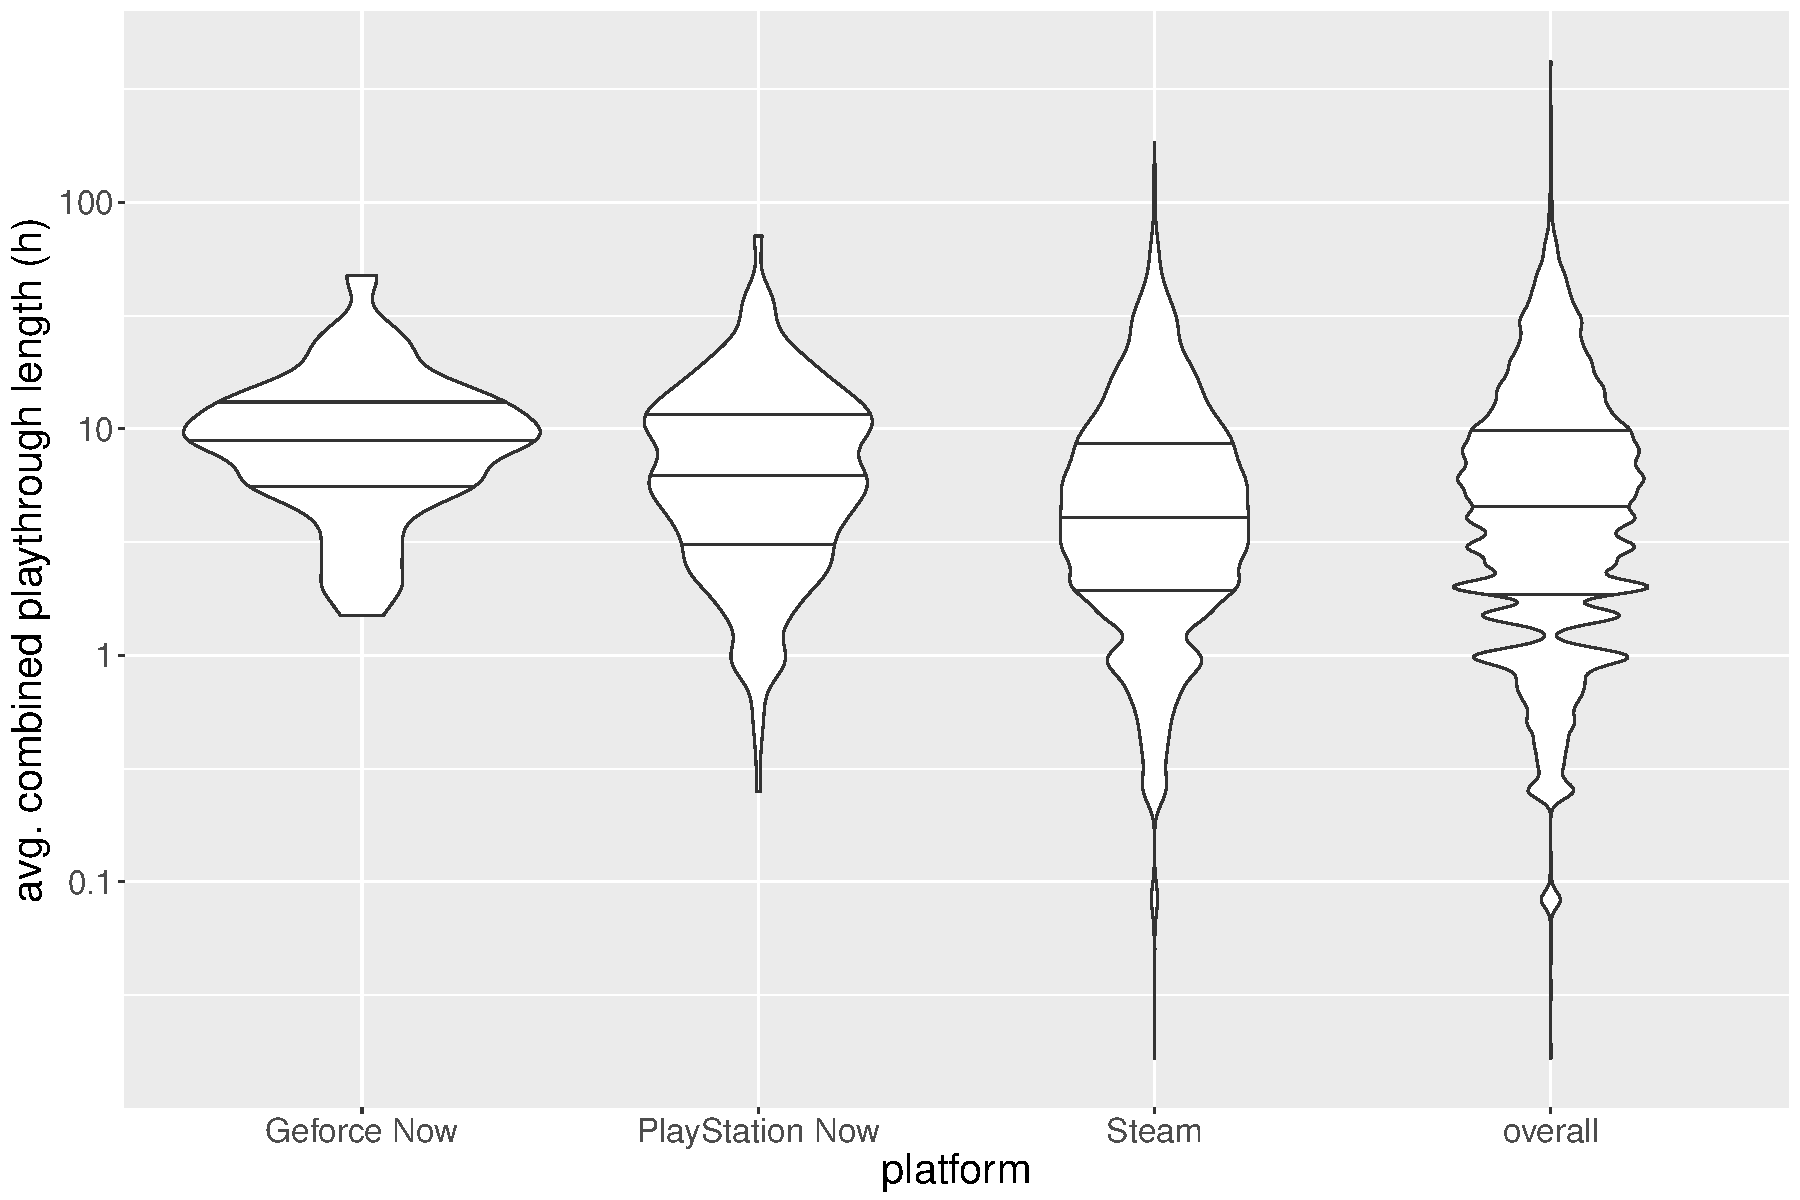
\includegraphics[width=1.0\columnwidth]{images/gamelengths-by-platform-violin.pdf}
	\caption{Violin plot of the per-platform average game lengths from \hltb. The number of games per bin are $68$, $209$, $7764$, and $18433$; quartiles indicated by horizontal lines.}
\label{fig:gamelengths-violin}
\end{figure}



%%%%%%%%%%%%
\subsubsection{Game Prices}

Trying to compare the prices per game is a difficult endeavor, due to the mixed approach of both cloud gaming platforms. The \gfnow subscription gives access to a subset of its catalog that can be extended by purchasing additional games. Similarly, \psnow has a base subscription catalog and additional, rent-able titles. But in addition, every title can also be rented without the need for an active subscription.
Nevertheless, for \steam it is possible to discuss unit prices: Using the official \acrshort{REST} \acrshort{API}, name and current price of each game were fetched at three different points in time\footnote{\url{https://github.com/mas-ude/steam-data-stats}}. This data was combined with \acrshort{API} data from the 3rd-party site \textit{SteamSpy}\footnote{\url{https://steamspy.com}}, which parses all publicly visible \steam user profiles. Subsequently, \textit{SteamSpy} estimates statistics on the size of the player base and the time each player spends with a title. Furthermore, the site provides a heuristic projection of the total number of owners of each listed title on \steam. Using the combined data, additional perspectives can be given.

\begin{table}
\centering
\caption{Average prices for \steam games.}
\label{tab:steam-price-stats}
\begin{tabu}{X[2]|X[r]X[r]X[r]}
	\toprule
	& \textbf{2015-07-14} & \textbf{2015-10-30} & \textbf{2016-02-06} \\
	\midrule
	\textbf{Portfolio price (€)} & $10.11$ & $8.47$ & $5.65$ \\
	\textbf{Weighted price (€)} & $12.39$ & $10.21$ & $5.30$ \\
	\bottomrule
\end{tabu}
\end{table}

Table~\ref{tab:steam-price-stats} shows the development of average \steam game prices for the three measurements taken. Two different types of averages are shown: The portfolio price which averages over all current game prices, and the weighted price which is the product of game price and estimated number of owners, averaged over the total number of games owned. Strong temporal effects are evident from either metric. Note that the last measurement shortly predates 2016's Lunar New Year, around which \steam ran a large seasonal sales campaign\footnote{\url{http://store.steampowered.com/news/20313/}}.

\begin{figure}[!t]
	\centering
	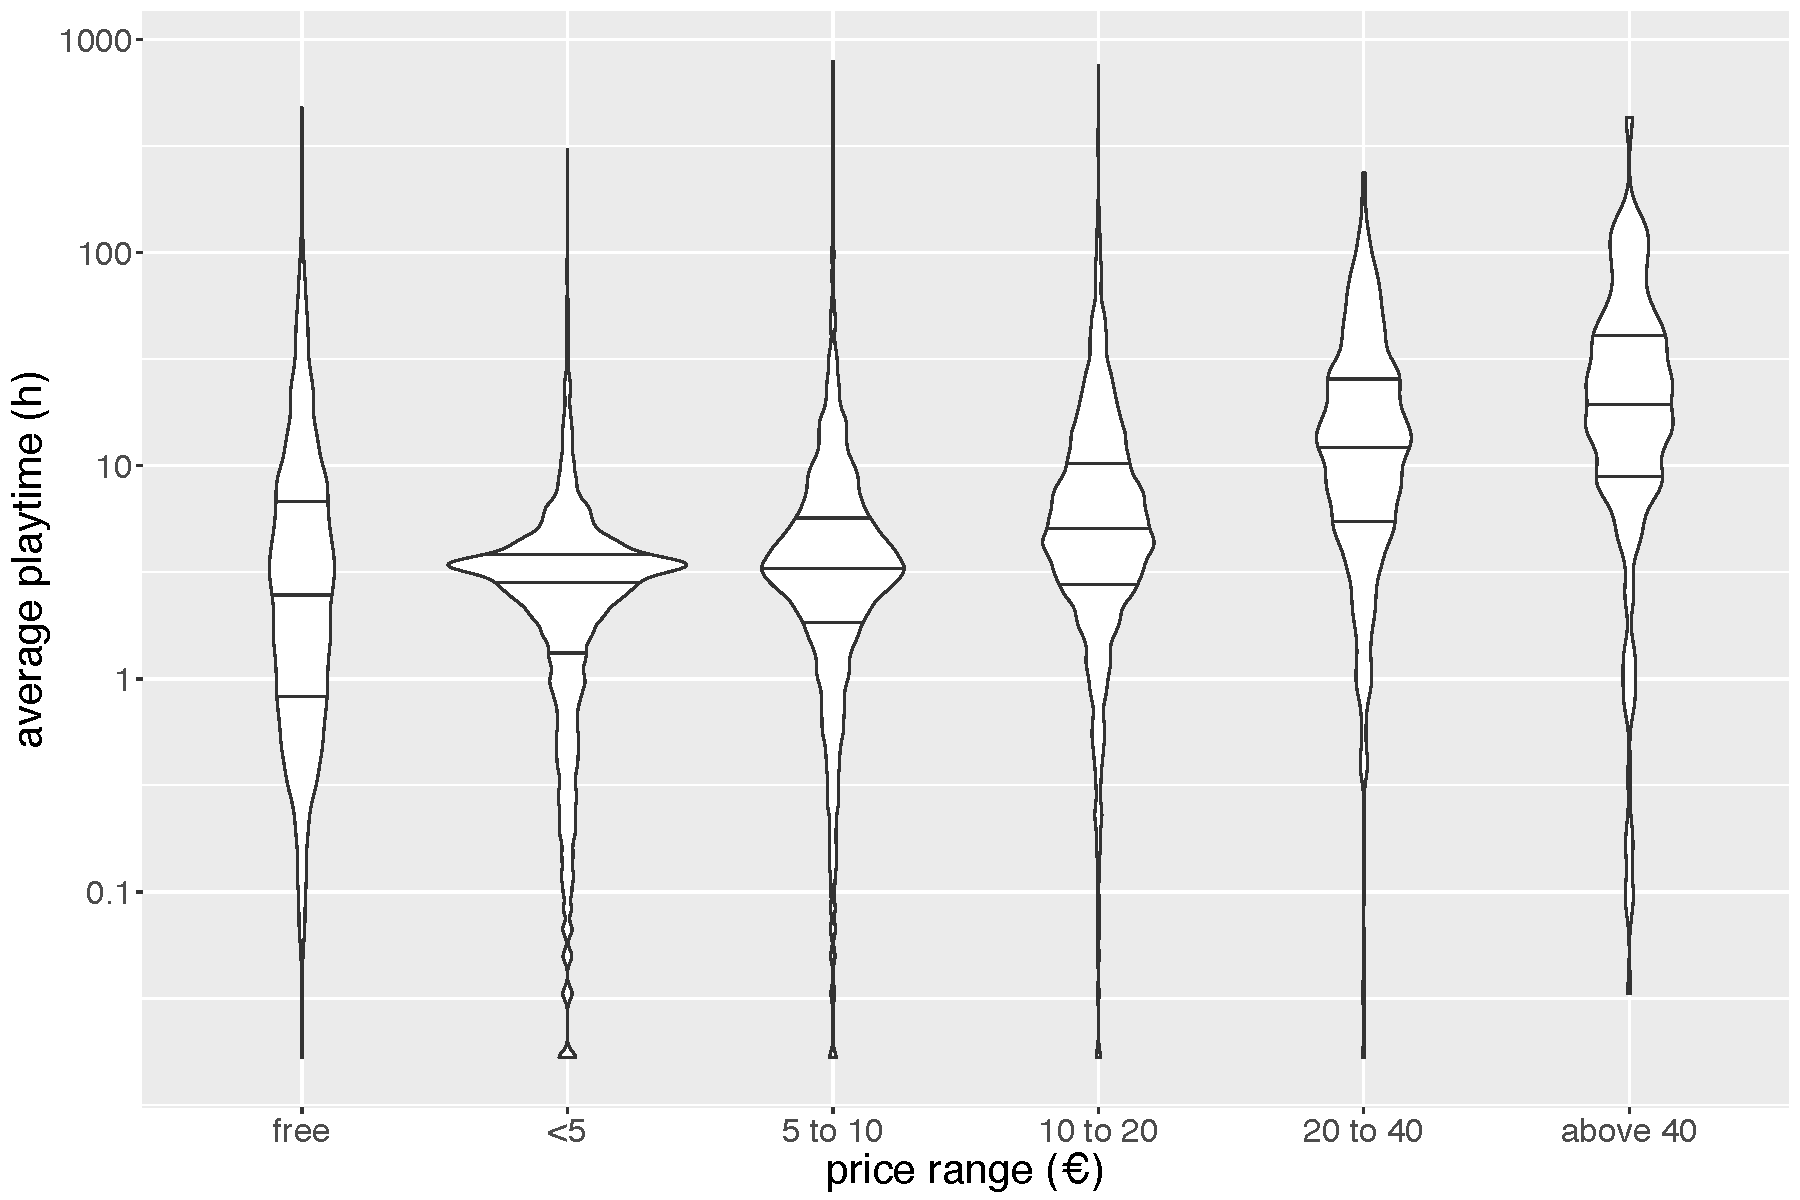
\includegraphics[width=1.0\columnwidth]{images/steam-cost-vs-playtime-non-sale.pdf}
	\caption{Violin plot of the average playtime of \steam games, broadly categorized by their prices. The number of games per bin are $1122$, $2177$, $1946$, $1106$, $328$, and $90$.}
\label{fig:steam-cost-vs-playtime-violin}
\end{figure}

Figure~\ref{fig:steam-cost-vs-playtime-violin} breaks down the distribution of average playtimes per game price range. The game price ranges are chosen so as to roughly separate the prevalent modes of the price distribution.
Playtime is defined as the time game owners spend playing a game, as recorded by the \steam platform and scraped from \textit{SteamSpy}. As can be seen, the playtimes generally increase with the price range; unfortunately, the data does not explain the cause: E.g., more expensive games might have more playable content, causing the playtime to increase. Conversely, higher upfront costs may incite players to spend more time regardless of game quality, thus avoiding regret for the expense. On the far left in the Figure, playtimes of ``free'' titles (including free-to-play games with monetization options other than an upfront payment) span almost the whole playtime range with less pronounced prevalences.
Due to the strong popularity of \steam in PC gaming (even physical retail copies often require using the service nowadays) this set also gives a good general overview of the dimensions of PC gaming in general.


%%%%%%%%%%%%
\subsubsection{Review Scores}

The final characteristic in this analysis are game review scores as given by professional gaming media outlets. This relies on the \metacritic dataset again. This set covers review scores for all current and historic gaming platforms. The review scores are aggregated to average scores ranging between $0$ and $100$. Some \metacritic-internal weighing factors are applied to express the importance of some media outlets over others.
The average scores seem quite similar across all services, albeit with a slightly lower $\sigma$ for \gfnow. Figure~\ref{fig:scores-by-platform} shows the distribution of review scores per platform. Both Cloud services seem to favor certain score levels. Specifically, their lowest quartiles (representing the worst-rated games on these platforms) reach much higher values than \steam's. This could be an effect of the Cloud systems curating the game offer to focus on highly-rated (and thus perhaps more attractive) titles. \steam on the other side is a more or less open platform, where every game publisher can sell their games at their own volition (platform operator collects a commission fee for sales). Consequently, it is reasonable to assume more variation in the quality of games, which could in turn lead to mixed reviews.

\begin{figure}[!t]
	\centering
	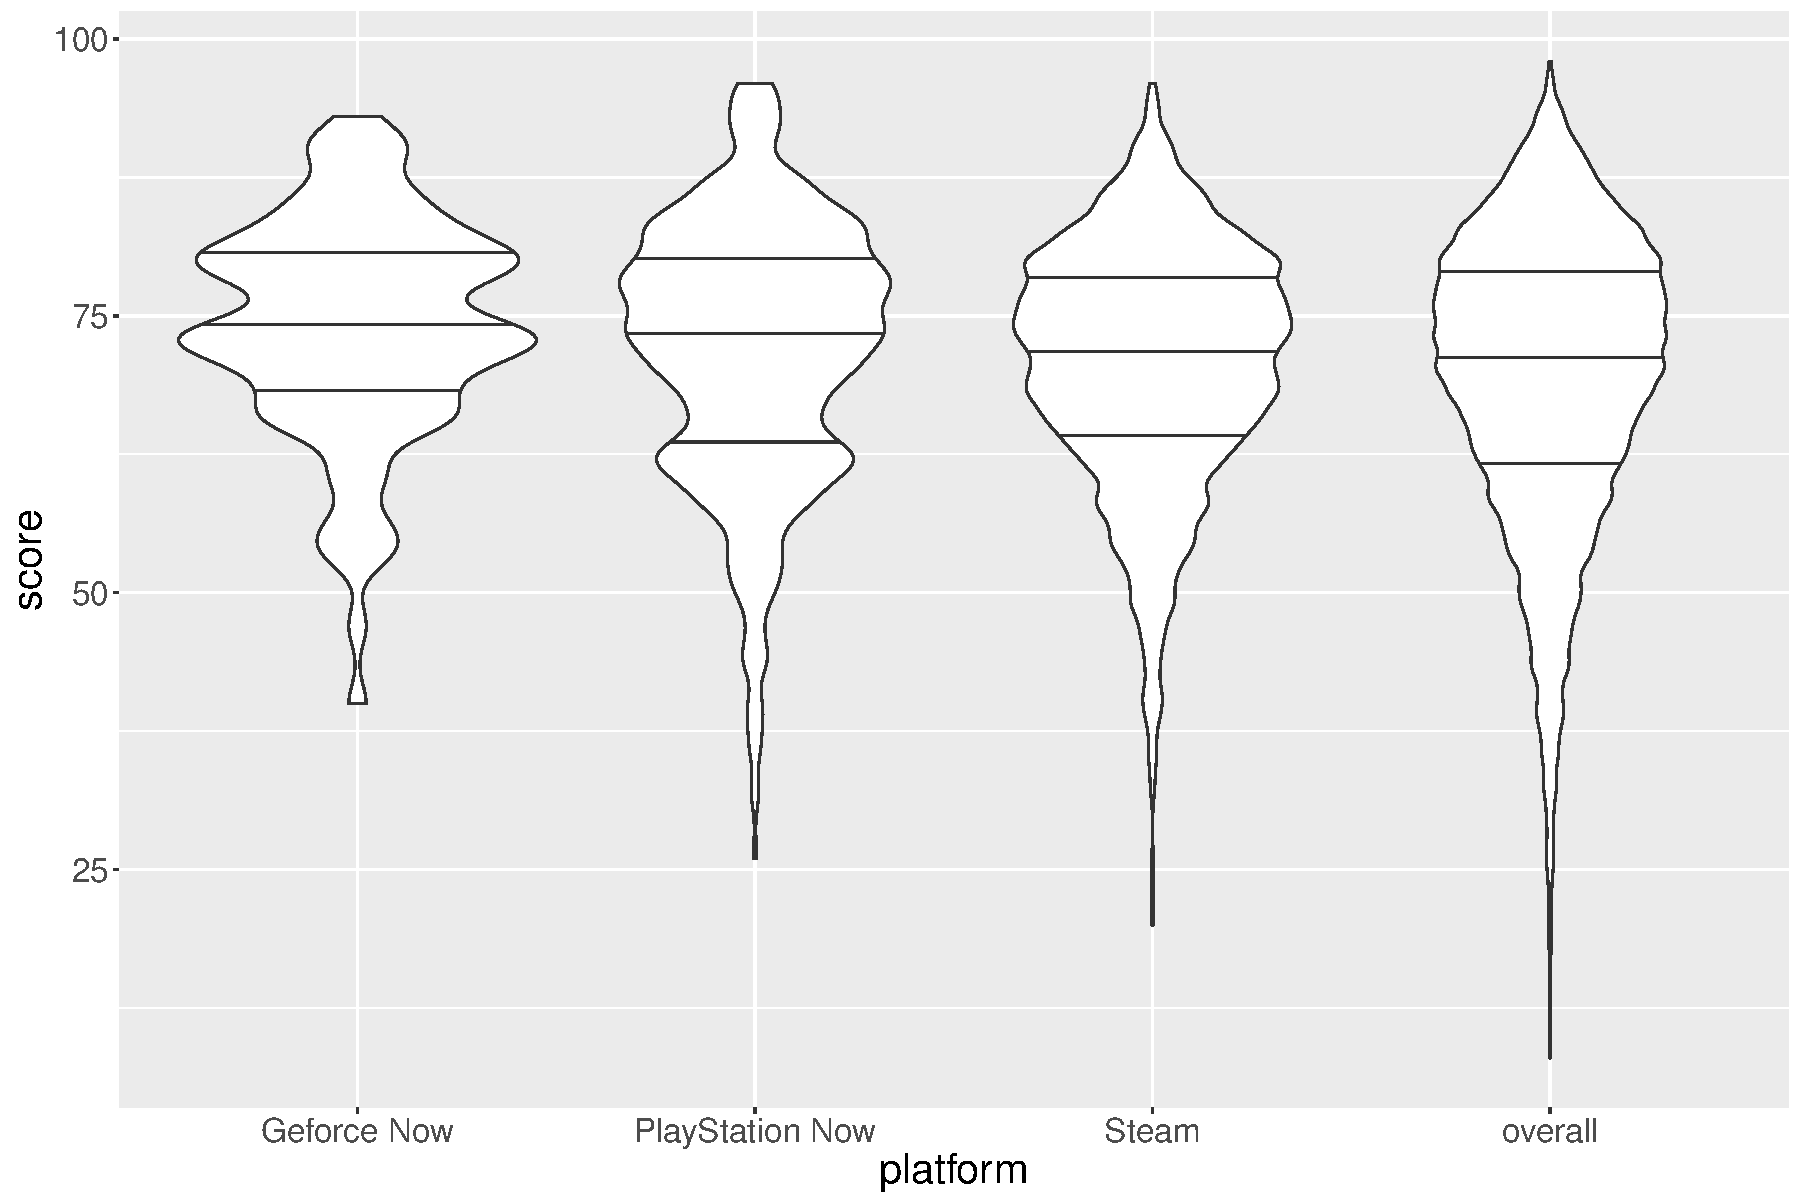
\includegraphics[width=1.0\columnwidth]{images/scores-by-platform-violin.pdf}
	\caption{Violin plot of aggregated review scores per platform. The number of games per bin are $68$, $209$, $7759$, and $46197$. Overall represents all games scraped from \metacritic.}
\label{fig:scores-by-platform}
\end{figure}


%!TEX root = paper.tex
%%%%%%%%%%%%%%%%%%%%%%%%%%%%%%%%%%%%%%%%%%%%%%%%%%%%%%%%%%%%%%%%%%%%%%%%%%%%%%%%
\section{Evaluation}
\label{sec:eval}

This section presents the results of the online survey
(\S~\ref{subsec:survey}) and
investigates the properties of the actual games offered on the
various platforms (\S~\ref{subsec:platformproperties}).
The survey covers context influence factors including social,
novelty and service-related ones. The platform study scrutinizes
service aspects.

\subsection{Online Survey Results}\label{subsec:survey}
The online survey was completed by $488$ participants
(\SI{91}{\percent} self-identified as male, \SI{8}{\percent} as female), reporting
ages between $13$ and $70$ years (quartiles $21$, $26$, $32$; mode $31$).
All responses were logged in a time frame of four days in early 2018.

\subsubsection{Gaming Demographics}
Around \SI{85}{\percent} of
participants started playing video games before they were ten years old.
Over \SI{50}{\percent} of participants play for $1$--$3$ hours per day.
\SI{44}{\percent} and \SI{36}{\percent} spend \$ $0$--$20$ and \$ $21$--$50$ on games per month, respectively.
Almost 50\% of participants own between $101$ and $500$ games, and about
15\% report to own $11$ to $50$ and $501$ to $1000$ games, respectively.
More than 40\% of participants bought $3$ to $10$ games in the last
twelve months; slightly more than 45\% claim to have bought
$10$ to $100$ games.



\subsubsection{Social Context Factors And Novelty}

When asked to mark all ways of learning about new games, respondents
most prevalently selected ``news on gaming sites'', ``reviews'', and
``friends'' (about \SI{60}{\percent} each). Other popular factors include
``live streams'', ``recommendations in online stores'', and
``gaming bundles'' (with \SI{40}{\percent}, \SI{30}{\percent}, and \SI{20}{\percent} each). Retail stores are hardly mentioned.
The popularity of games on \textit{Twitch} (a website dedicated to
live streaming of video games) or with game critics is judged as not
important to over \SI{70}{\percent} and over \SI{60}{\percent} of participants, respectively.

\subsubsection{System Influence Factors}
Almost all participants (\SI{97}{\percent}) own a PC, the two other most prevalent
gaming systems are smartphones (\SI{30}{\percent}) and Sony's PlayStation 4 (\SI{26}{\percent}).
Nintendo's Switch and 3DS as well as Microsoft's XBox One are reported
by between \SI{18}{\percent} and \SI{11}{\percent} of participants.
\SI{93}{\percent} report the PC to be their favorite gaming system, with consoles
favored by \SI{29}{\percent}.



\subsubsection{Service Factors}

Digital gaming stores (and among these, \steam) are reported as
the most popular ways of obtaining games. About \SI{85}{\percent} of respondents
use digital storefronts. The other proposed selections reach far lower
values: ``third-party key sellers'' hits \SI{35}{\percent}, and both ``physical
games from online stores'' and ``physical games from retailers''
are capped around \SI{25}{\percent}.
90\% of participants use the \steam platform; \textit{Humble Bundle}
and \textit{GOG} are very popular (almost \SI{60}{\percent}) as well. \textit{Origin}
at \SI{38}{\percent} is a relatively distant fourth already. None of the other
proposed selections, including the console-specific digital stores
(PlayStation Network/Store, Nintendo eShop, XBox Store), exceed
\SI{25}{\percent}.

Figure~\ref{fig:buying-factors} shows the respondents' assessments
of factors important for buying new gaming systems, grouped by
importance. As can be seen, system prices are a motivator for
almost \SI{70}{\percent} of survey participants. Online multiplayer capabilities,
system-exclusive games, and graphics are important or very important
for more than \SI{40}{\percent}, each. On the other side, local multiplayer
capabilities, the mere recency of games, and available downloadable
content are deemed relatively unimportant factors for a buying decision.

The survey also asked about buying hindrances for newly released 
games, i.e. reasons that speak against buying them.
More than \SI{70}{\percent} of participants declare a lack of interest
that hinders them. Financial reasons play a role for roughly
a third of respondents, and a similar proportion has a substantial
backlog of games awaiting to be played, whereas only \SI{15}{\percent} declared
their hardware to be lacking support for the latest games.


\begin{figure}[!t]
	\centering
	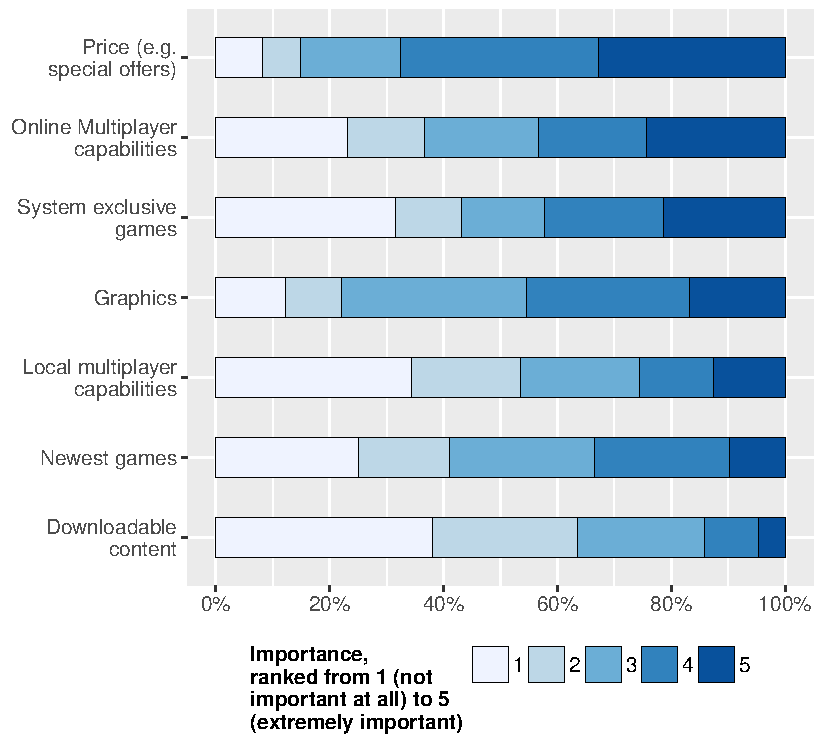
\includegraphics[width=1.0\columnwidth]{images/buyingfactors.pdf}
	\caption{Respondents' assessment of factors important for buying
	new gaming systems.}
\label{fig:buying-factors}
\end{figure}


\subsection{Game Platform Properties}\label{subsec:platformproperties}

To complement the subjective gamer results and also provide an
inter-platform comparison, the attention now turns to the service
factors of three gaming platforms: \steam, \gfnow, and \psnow.
Table~\ref{tab:game-stats} provides an overview of the data
collected, showing the number, age, length, and review scores
across platforms.

%%%%%%%%%%%%

\begin{table*}
\centering
\caption{Game characteristics on the investigated platforms. Title counts from Web/API scraping, lengths from \hltb, ages and review scores from \metacritic.}
\label{tab:game-stats}
	\begin{tabu}{X[2]|X[r]X[r]X[r]X[r]X[r]X[r]X[r]}
	\toprule
	Service & Titles & Age $\mu$ & Age $\sigma$ & Length $\mu$ & Length $\sigma$ & Score $\mu$ & Score $\sigma$ \\
	\midrule
	\gfnow & $118$ & \SI{3.1}{\year} & \SI{\pm2.3}{\year} & \SI{10.7}{\hour} & \SI{\pm8.2}{\hour} & $73.9$ & $\pm10.1$ \\
	\psnow & $432$ & \SI{4.8}{\year} & \SI{\pm2.4}{\year} & \SI{8.8}{\hour} & \SI{\pm8.8}{\hour} & $71.9$ & $\pm12.0$ \\
	\steam & $14,120$ & \SI{2.5}{\year} & \SI{\pm3.3}{\year} & \SI{7.3}{\hour} & \SI{\pm10.2}{\hour} & $70.6$ & $\pm11.0$ \\
	\bottomrule
	\end{tabu}
\end{table*}


%%%%%%%%%%%%
\subsubsection{Number of Games}

The two cloud
platforms offer a very limited number of games when compared to the
games available on \steam, which itself again only represents a subset
of all games available either on the PC platform (\metacritic lists
\num{26420}) or across all platforms (\num{57308}). Two
possible, simple explanations for the low game count on the cloud
platforms come to mind: One is that they were launched relatively
recently (2015) in comparison to \steam (2003), leaving little time for
the range of games to grow. Secondly, the choice of games for a cloud
gaming platform is most likely curated by the platform operator for
compatibility and performance reasons. This usability burden shifts to
the end user for digital storefronts like \steam, allowing these
platforms to offer a larger variety of games, including ones that are
very demanding on the hardware.


%%%%%%%%%%%%
\subsubsection{Game Ages}

The average
game ages appear to be relatively high for all of the investigated
platforms, and particularly so for \psnow. It might be considered a
special case, as it is specifically advertised as a backwards
compatibility for older, pre-PlayStation 4 games that do not run on the
latest Sony platform any more. For \steam, the distribution is
significantly skewed towards recent titles: A quarter of games are less
than a year old, and the median is at $21$ months. The
distribution's tail extends beyond $25$ years due to re-releases
of ``classic'' games on the platform.


%%%%%%%%%%%%
\subsubsection{Game Lengths}
Figure~\ref{fig:gamelengths-violin} shows the distribution of aggregated
game lengths for the three platforms under investigation, and an
``overall'' distribution that includes further platforms and gaming
systems. Among the three platforms, the median reported game
length is largest for \gfnow. In
contrast to the curated choice of games on the Cloud systems, \steam
also offers shorter and longer games.

\begin{figure}[!t]
	\centering
	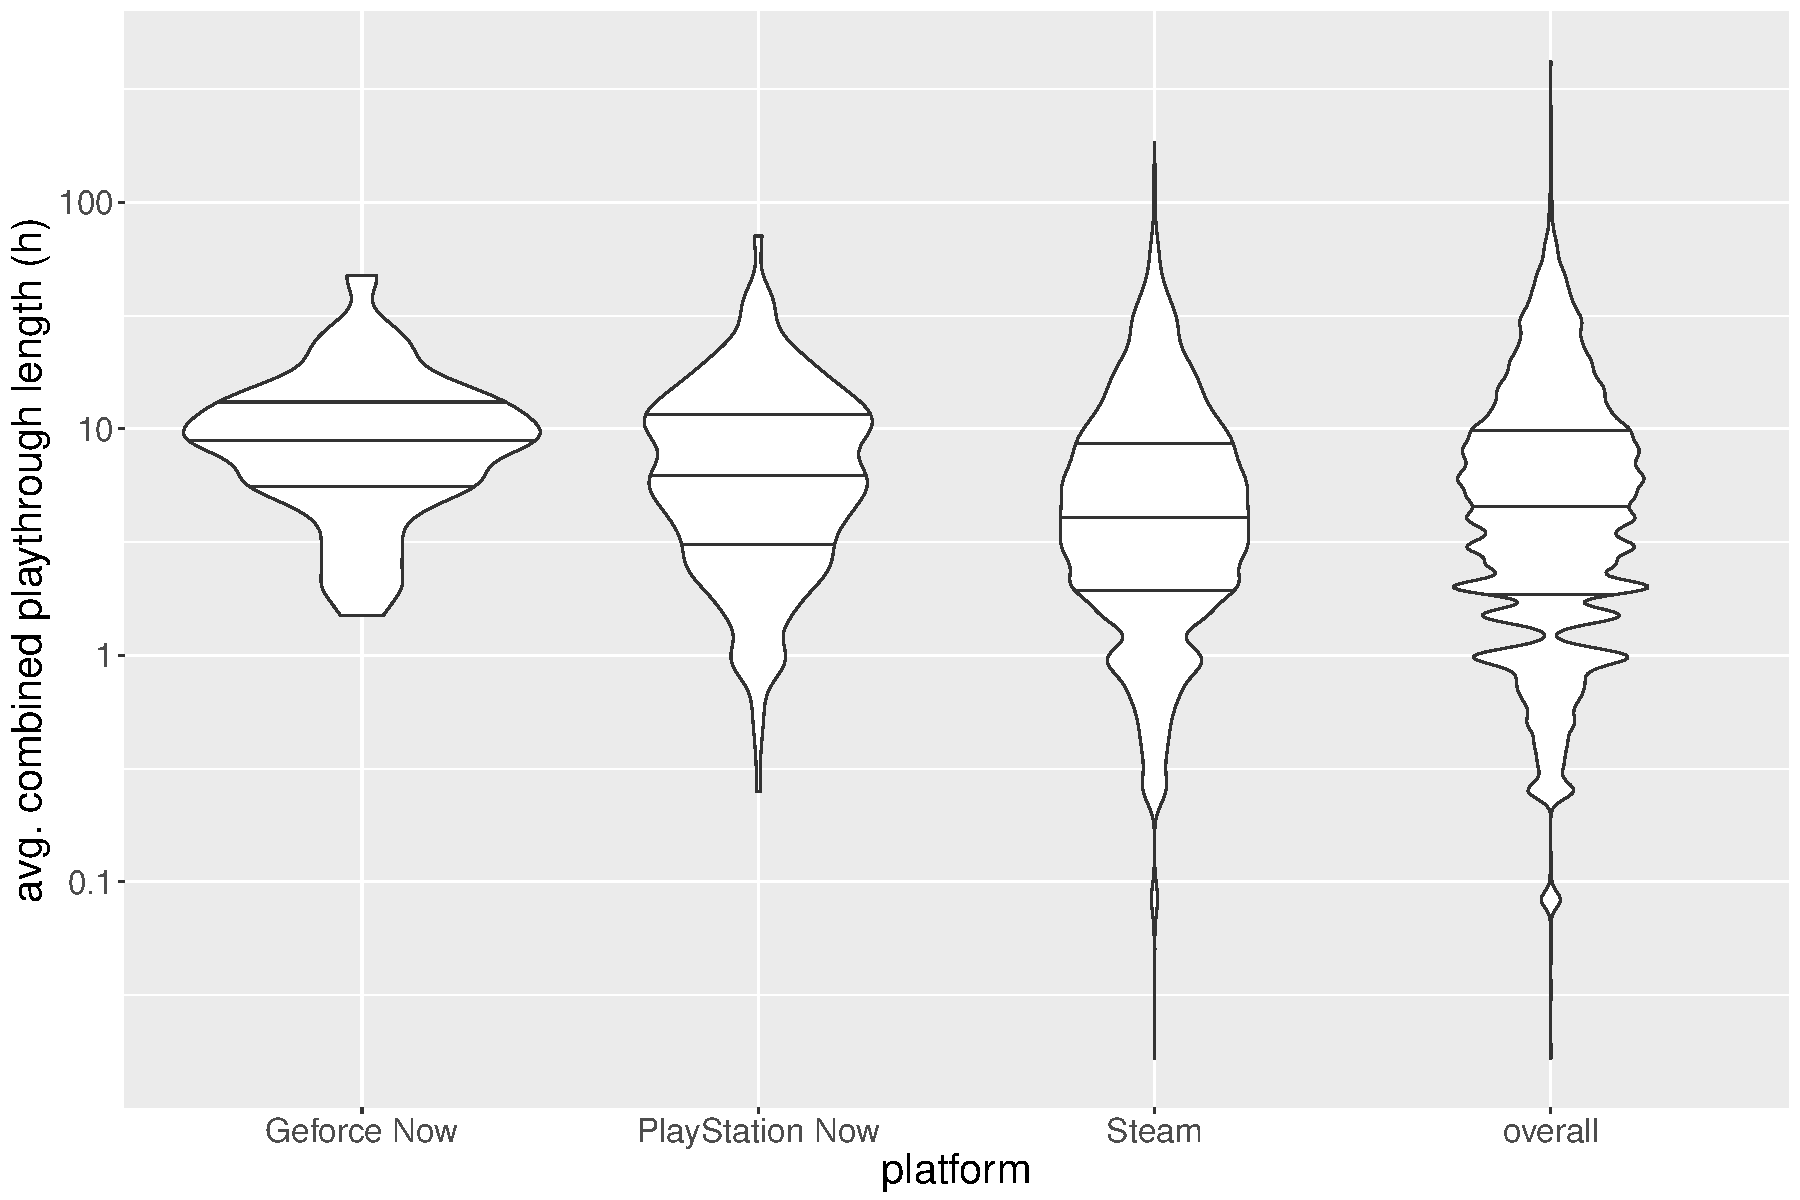
\includegraphics[width=1.0\columnwidth]{images/gamelengths-by-platform-violin.pdf}
	\caption{Violin plot of the per-platform average game lengths from \hltb. Quartiles indicated by horizontal lines.}
\label{fig:gamelengths-violin}
\end{figure}


%%%%%%%%%%%%
\subsubsection{Game Prices}

Trying to compare the prices per game is a difficult endeavor, due to
the mixed approach of the gaming platforms. The \gfnow subscription
gives customers access to a subset of its catalog that can be
extended by purchasing additional games; \gfnowpc 
on the other hand requires the customer to buy games on their
own and pay for the time spent playing.
\psnow and \psnowpc have a flat rate for all of their catalog.
At least for \steam, unit prices can be discussed.
Between mid-2015 when the authors started monitoring \steam's catalog,
and late 2017 when the last measurement was taken,
its average price has decreased from \SI{10.11}[\$]{} to \SI{8.83}[\$]{}. In the same
timeframe, the number of games more than doubled, from \num{5996} to
\num{14120}. The prices vary a lot over time, for instance due to
seasonal sales periods.

\begin{figure}[!t]
	\centering
	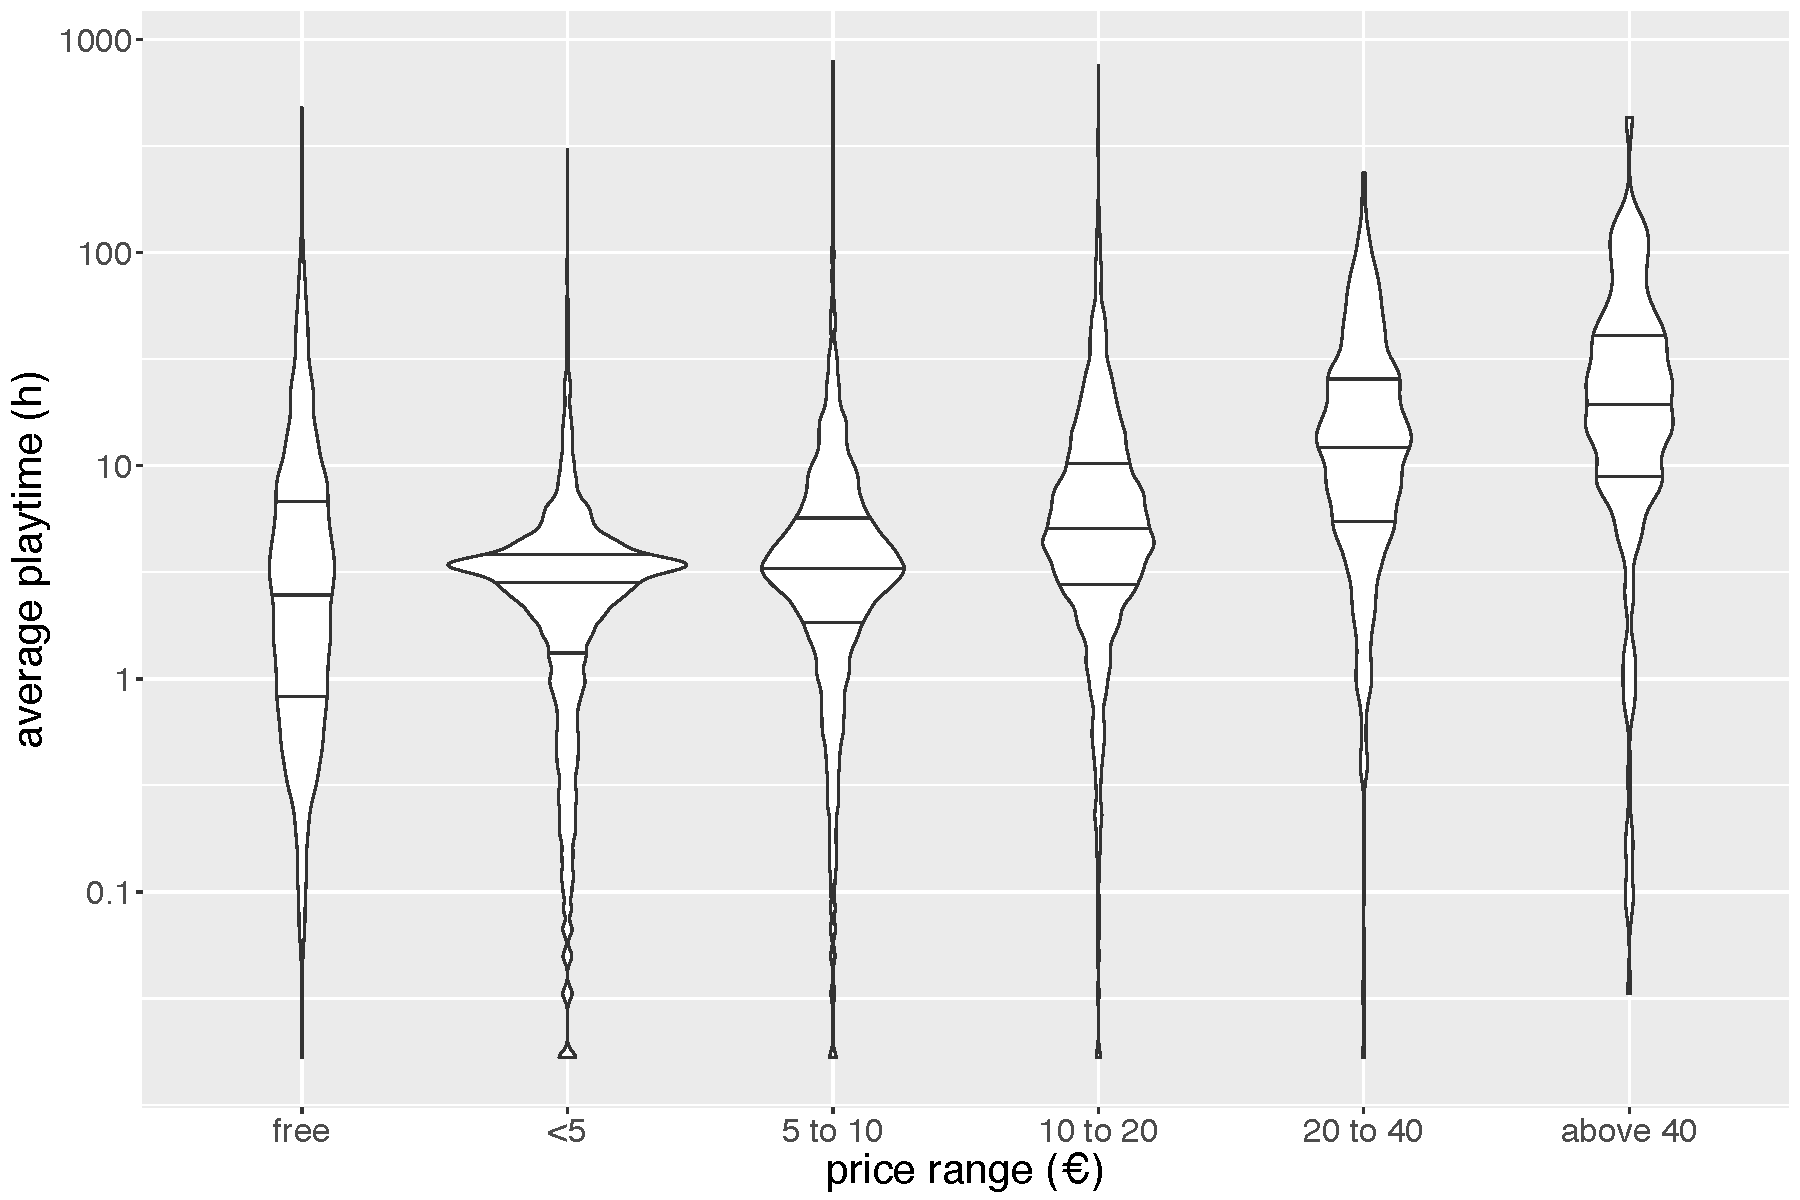
\includegraphics[width=1.0\columnwidth]{images/steam-cost-vs-playtime-non-sale.pdf}
	\caption{Violin plot of the average playtime of \steam games, broadly categorized by their price ranges. The number of games per bin are $1541$, $5269$, $4019$, $2445$, $658$, and $188$. Quartiles indicated by horizontal lines.}
\label{fig:steam-cost-vs-playtime-violin}
\end{figure}

\subsubsection{Price versus Playtime}
Again focusing on \steam,
Figure~\ref{fig:steam-cost-vs-playtime-violin} breaks down the
distribution of average playtimes per game price range. The game price
ranges are chosen so as to roughly separate the prevalent modes of the
price distribution.
Playtime is defined as the time game owners spend playing a game, as
recorded by the \steam platform and scraped from \textit{SteamSpy}.
Playtimes of ``free'' titles 
span almost the whole playtime range.
For games that cost less than \SI{5}[\EUR]{}, the mode is around
\SI{3.5}{\hour} of playtime, and values are concentrated around it.
This recent trend only
manifested itself in datasets in the last twelve months: 
The number of games in this price category grew by a factor of
$2.4$ in that timeframe, whereas they
increased by only \SI{37}{\percent} in the free price range, and roughly doubled
in the other price ranges.

Other than that, the median playtime increases with the price range;
unfortunately, the data does not explain the cause: E.g., more expensive
games might have more playable content, causing the playtime to
increase. Conversely, higher upfront costs may incite players to spend
more time regardless of game quality, thus avoiding regret for the
expense.


%%%%%%%%%%%%
\subsubsection{Review Scores}

The final characteristic presented from the data are game review scores as
given by professional gaming media outlets. This relies on the
\metacritic dataset. This set covers review scores for all current
and historic gaming platforms. The review scores are aggregated to
average scores ranging between $0$ and $100$. Some \metacritic-internal
weighing factors are applied to express the importance of some media
outlets over others.
The average scores exceed $70$ across all services, albeit with a
slightly lower $\sigma$ for \gfnow.



\subsection{Subjective Assessments Of Utility Metrics}

Finally, the survey also included questions that directly target
the utility metrics of platforms described above.
To put prices and playtimes into perspective, the survey asked
whether $5$ to $10$ hours of gameplay were enough for a price of \SI{60}[\$]{}.
More than \SI{50}\% of participants strongly disagreed, and more than
\SI{20}{\percent} disagreed. This demand-side rejection clearly fits the picture of
Figure~\ref{fig:steam-cost-vs-playtime-violin}, where less than a
quarter of games that cost more than \SI{40}[\EUR]{} are played for less than
$10$ hours.

The absence of game recency as a motivational factor was discussed
above already; other motivational factors that respondents strongly
agreed to were preferences of gameplay over graphics, and gaming
experience in general (both reaching almost \SI{80}{\percent} importance ratings).
Also, over half of the respondents value replayability, i.e. to
be able to play a game more than once.

A result relevant for the curated offers of \gls{cg}
platforms is that almost \SI{80}{\percent} or respondents are not interested in
exchanging flat-rate access fees for buying individual games.
Other responses from survey participants indicate a multitude of
interests and motivations for and against platforms, including
statements like ``I buy only games with Linux support'',
or hints at the availability of ``pirated'' games.

%!TEX root = paper.tex
%%%%%%%%%%%%%%%%%%%%%%%%%%%%%%%%%%%%%%%%%%%%%%%%%%%%%%%%%%%%%%%%%%%%%%%%%%%%%%%%
\section{Conclusion}
\label{sec:conclusion}

While cloud gaming is a topic of strong interest, it comes with a series of problems and limitations, both of technical and economic nature. Our user-side analysis makes apparent the curated nature of current cloud gaming services which entails a narrow offer of hand-selected games and sometimes even a narrow target group (see the case of \psnow). This naturally limits the value of a subscription-based service model for customers, when insufficient convenience and price advantages can be yielded.

In addition to that, the operator-side also reveals major issues due to the need for highly regional data-centers and specialized hardware. This eliminates any chance for the efficiency gains that general cloud services are intended for. Moreover, subscription-based models suffer from the expected higher peak utilization in comparison to à la carte game purchasing models, which creates a high cost pressure due to enormous infrastructure investments and limited scaling advantages.

However, there might be some niches for specific games or audiences that could be sustained at reduced operational efforts. This might be an angle worth of investigation in the future, especially with better engagement metrics and more detailed models of gaming data center operations. Another economically more feasible alternative to cloud gaming could be game streaming in the local network. This option would still require all the usual gaming hardware and services like \steam but would bring all the convenience and flexibility of cloud gaming.


\printbibliography

\balance

\end{document}
